\chapter{Functional Methods}
\label{chapter:functional-methods}

In this Chapter, the basic theoretical tools of this work are introduced briefly. Functional methods, such as the DSEs or the fRG, provide non-perturbative relations for the full correlation functions of a quantum field theory. For more detailed reviews, see~\cite{Swanson2010} (DSEs) and~\cite{Kopietz2010,Pawlowski2007} (fRG). In the following, we will put emphasis on Dyson-Schwinger equations and field theories at finite temperature. At the end of this Chapter, we discuss the spectral representation.

\section{Dyson-Schwinger equations}
\label{section:dyson-schwinger-equations}

Functional methods are based on the path integral formulation of QFT. In general, a QFT is described by the microscopic action $S[\phi]$. Analogously to statistical physics, the generating functional $Z[J]$ can be written in Euclidean spacetime as
%
\begin{align}
	\label{eq:generating-functional}
	Z[J] = \frac{1}{\mathcal{N}} \int \mathcal{D}\phi\; \mathrm{e}^{-S[\phi]+J\cdot\phi} \quad \mathrm{with} \quad J\cdot\phi\equiv\int_x\;J(x)\phi(x)\,,
\end{align}
%
where $\mathcal{N}$ is a normalization constant, $J(x)$ is some external source field, and $\int\mathcal{D}\phi$ is the functional integral over all possible field configurations $\phi$. The correlation functions are then obtained by functional derivatives with respect to the source fields,
%
\begin{align}
	\label{eq:correlation-functions}
	\langle \phi(x_1)\dots\phi(x_n)\rangle = \frac{1}{Z[0]}\frac{\delta^n Z[J]}{\delta J(x_1)\dots\delta J(x_n)} \Bigg|_{J=0} \,.
\end{align} 
%
By the reconstruction theorem, a quantum field theory is completely determined by its correlation functions~\cite{Wightman1956}. Thus, the path integral contains the full information of the theory. 
However, it can be shown that the correlation functions in Eq.~\eqref{eq:correlation-functions} contain redundant information and can be split into a connected and disconnected part. In case of a two-point function~\cite{Peskin1995},
%
\begin{align}
	\label{eq:two-point-function}
	\langle \phi(x_1)\phi(x_2)\rangle = \langle \phi(x_1)\phi(x_2)\rangle_c + \langle\phi(x_1)\rangle\langle\phi(x_2)\rangle \,,
\end{align}
%
where $c$ denotes the connected part of the correlation function in which all external lines of the Feynman diagrams are connected. This redundancy is removed by the Schwinger functional $W[J]$, which generates only connected correlation functions,
%
\begin{align}
	\label{eq:schwinger-functional}
	W[J] = \ln Z[J] \,.
\end{align}
%
In particular, the full propagator is defined by the connected two-point function~\cite{Peskin1995},
%
\begin{align}
	\label{eq:propagator-schwinger}
	G(x_1,x_2) = \langle \phi(x_1)\phi(x_2)\rangle_c = \frac{\delta^2 W[J]}{\delta J(x_1)\delta J(x_2)} \Bigg|_{J=0} \,,
\end{align}
%
and can be obtained by Dyson resummation of amputated one-particle-irreducible (1PI) contributions. Here, 1PI refers to Feynman diagrams which cannot be divided into two separate diagrams by cutting one internal line. 

Thus, the entire information of the theory is already encoded in the 1PI diagrams. The generating functional of 1PI correlation functions is the quantum effective action $\Gamma[\Phi]$, which is defined as the Legendre transform of the Schwinger functional,
%
\begin{align}
	\label{eq:effective-action}
	\Gamma[\Phi] = \sup_J\big[J\cdot\Phi - W[J]\big] = J_{\sup}\cdot\Phi - W[J_{\sup}] \,,
\end{align}
%
where $\Phi=\langle\phi\rangle$ is now the mean field and $J_{\sup} = J_{\sup}[\Phi]$ is the field-dependent current that minimizes~\eqref{eq:effective-action}. From a physical point of view, the effective action $\Gamma$ is the quantum analogue of the classical action $S$, which accounts for all quantum corrections. A non-perturbative connection between the quantum and classical equations of motion is provided by the Dyson-Schwinger equation (DSE)~\cite{Dyson1949,Schwinger1951},
%
\begin{align}
	\label{eq:DSE}
	\frac{\delta\Gamma}{\delta\Phi}\left[\Phi\right] = \frac{\delta S}{\delta\phi}\left[\phi=\Phi+G\cdot\frac{\delta}{\delta\Phi}\right] \,,
\end{align}
%
which follows from the shift independence of the path integral measure. A more detailed derivation and discussion can be found in~\cite{Pawlowski2021}. The product in the argument of Eq.~\eqref{eq:DSE} is defined by
%
\begin{align}
	\label{eq:propgator-derivative}
	G\cdot\frac{\delta}{\delta\Phi} = \int_x G(x_1,x)\cdot\frac{\delta}{\delta\Phi(x)} \,.
\end{align}
%
All higher order 1PI correlation functions are obtained by functional derivatives with respect to the mean field $\Phi$,
%
\begin{align}
	\label{eq:1PI-correlation-functions}
	\Gamma^{(n)}(x_1,\dots,x_n)=\frac{\delta^n\Gamma[\Phi]}{\delta\Phi(x_1)\dots\delta\Phi(x_n)} \,.
\end{align}
%
It can be shown that the two-point function is exactly the inverse of the full propagator,
%
\begin{align}
	\label{eq:propagator-gamma}
	\Gamma^{(2)}(x_1,x_2) = G^{-1}(x_1,x_2) \,.
\end{align}
%
Note that this is a matrix equation in general. Thus, the inversion must account for all off-diagonal terms. In the following, we summarize the main extensions when dealing with multiple fields of different species.

For a general set of fermionic and bosonic fields, one can introduce a superfield $\Phi$ which collects all field indices and species. In case of ultracold Fermi gases, the superfield is given by $\Phi=(\psi_{\sigma},\psi_{\sigma}^*,\phi,\phi^*)$ with fermion species $\sigma=(\uparrow,\downarrow)$. The Dyson-Schwinger equation takes the form
%
\begin{align}
	\label{eq:DSE-general}
	\frac{\delta\Gamma}{\delta\Phi_a}\left[\Phi\right] = \frac{\delta S}{\delta\phi_a}\left[\phi_b=\Phi_b+G_{bc}\cdot\frac{\delta}{\delta\Phi_c}\right] \,,
\end{align}
%
where a sum over repeated indices is implied. Correlation functions are denoted by
%
\begin{align}
	\label{eq:super-correlation-functions}
	\Gamma^{(n)}_{\Phi_{a_1}\dots\Phi_{a_n}}=\frac{\delta}{\delta\Phi_{a_1}}\dots \frac{\delta}{\delta\Phi_{a_n}}\, \Gamma[\Phi] \,.
\end{align}
%
Finally, derivatives of propagators with respect to the mean fields are given by~\cite{Pawlowski2021}
%
\begin{align}
	\label{eq:derivative-propagator}
	\frac{\delta}{\delta\Phi_a} G_{bc} = -(-1)^{ab}(-1)^{ee} \, G_{bd}\cdot\Gamma^{(3)}_{dae}\cdot G_{ec} \,,
\end{align}
%
where $(-1)^{ab}=-1$, if $a$ and $b$ are fermionic, and $(-1)^{ab}=1$ otherwise. The relation between propagator and two-point function becomes $G_{ac}\cdot\Gamma^{(2)}_{cb}=(-1)^{ab}\delta_{ab}$.

This summarizes all necessary identities to work with functional methods in arbitrary theories involving fermions and bosons.

\section{Finite temperature and density}
\label{section:finite-temperature-density}

For a quantum field theory in thermal equilibrium, finite temperature can be introduced in analogy to classical statistical physics via the so called Matsubara formalism. More general approaches using e.g. Schwingers closed time path can be found in~\cite{LeBellac1996}. Here, we are mainly interested in the implications for the calculation of Feynman diagrams. 

In classical statistical physics, inverse temperature $\beta=1/T$ is the prefactor in front of the Hamiltonian in the partition function and can be viewed as a finite extent along imaginary times with $\tau=i\beta$. As a consequence, the imaginary time direction is compactified to the interval $\tau\in[0,\beta]$ and bosonic fields $\phi$ have to be periodic with period $\beta$, i.e.
%
\begin{align}
	\label{eq:periodic-condition}
	\phi(\tau+\beta,\bm{x})=\phi(\tau,\bm{x}) \,.
\end{align}
%
The finite temperature path integral can written as
%
\begin{align}
	\label{eq:finite-temperature-path-integral}
	Z = \int_{\phi(\beta,\bm{x})=\phi(0,\bm{x})} \mathcal{D}\phi\; \mathrm{e}^{-S[\phi]} \quad \mathrm{with} \quad S[\phi]=\int_0^{\beta}d\tau\int d^3x\, \mathcal{L}[\phi] \,,
\end{align}
%
where $\mathcal{L}$ is the imaginary-time (Euclidean) Lagrangian of the theory. The finite extent of the imaginary time axis and the periodic boundary condition have important consequences for the Fourier transform of fields,
%
\begin{align}
	\label{eq:matsubara-fourier-transform}
	\phi(\tau,\bm{x}) = T\sum_{\omega_n}\int\frac{d^3p}{(2\pi)^3}\, e^{-i(\tau\omega_n-\bm{x}\cdot\bm{p})}\, \phi(\omega_n,\bm{p})  \,,
\end{align}
%
where $\omega_n=2\pi n T$ with $n\in\mathbb{Z}$ are the so called Matsubara frequencies. Thus, the zero component of the momentum becomes discrete and the continuous integral turns into an infinite Matsubara sum, which can be evaluated using the residue theorem from complex analysis. To summarize, for the transformation of a QFT in vacuum to a QFT at finite temperature, one needs to perform the following replacement in appearing momentum integrals
%
\begin{align}
	\label{eq:finite-temperature-integrals}
	\int\frac{d^dp}{(2\pi)^d} \rightarrow T\sum_{\omega_n}\int\frac{d^{d-1}p}{(2\pi)^{d-1}}  \,.
\end{align}
%
In case of fermionic fields $\psi$, the path integral has to fulfill anti-periodic instead of periodic boundary conditions, i.e. $\psi(\tau+\beta,\bm{x})=-\psi(\tau,\bm{x})$. The Matsubara frequencies are given by $\omega_n=(2n+1)\pi T$ with $n\in\mathbb{Z}$.

The inclusion of a finite chemical potential $\mu$ leads to a finite density and follows also from the path integral in analogy to the grand canonical ensemble. Recall that the particle number is related to the chemical potential via derivative of the grand potential with respect to $\mu$. In order to include a chemical potential in the path integral, we add the respective term to the Euclidean action. In frequency space, this amounts to the following shift into the complex plane
%
\begin{align}
	\label{eq:chemical-potential}
	\omega_n \rightarrow \omega_n - i\mu \,.
\end{align}
%
Note that finite temperatures or densities break Lorentz and Galilei invariance in general, since they single out a specific frame of reference.

\section{Spectral representation}
\label{section:spectral-representation}

The spectral representation of the propagator plays a central role in the spectral functional approach. Usually, computations are performed in imaginary-time on discrete Matsubara frequencies $\omega_n$ which results in an ill-defined problem when analytically continuing to the real frequency axis, see Fig.~\ref{fig:spectral-properties}. In the present work, we assume the following Källén-Lehmann representation of the full propagators~\cite{Abrikosov1975,Fetter1971,Haussmann2009}
%
\begin{align}
	\label{eq:spectral-representation}
	G(\omega_n,\bm{p}) = \int_{-\infty}^{\infty} d\lambda \, \frac{\rho(\lambda,\bm{p})}{-i\omega_n+\lambda} \,,
\end{align}
%
where $\rho$ is the spectral function. In this way, the propagator is a symbolic expression in $\omega_n$ which can be evaluated at arbitrary frequencies in the complex plane. Physically, the spectral function acts as a linear response function of the propagator, encoding the energy spectrum of the theory, see also Fig.~\ref{fig:spectral-properties}. Eq.~\eqref{eq:spectral-representation} leads to the following inverse relation between the spectral function and the retarded propagator,
%
\begin{align}
	\label{eq:spectral-relation}
	\rho(\omega,\bm{p}) = \frac{1}{\pi}\, \mathrm{Im}\, G^R(\omega,\bm{p}) \,,
\end{align}
%
where $G^R(\omega,\bm{p})=G(-i(\omega+i0^+),\bm{p})$ and $\omega$ is now a real frequency. The existence of a spectral representation restricts all
non-analyticities of the propagator to lie on the real
frequency axis. For a more detailed discussion on the analytic properties, see~\cite{Perali2002,Rohe2001,Wink2020}. The fermionic spectral function satisfies the sum rule~\cite{Fratini2013}
%
\begin{align}
	\label{eq:spectral-sum-rule}
	\int_{-\infty}^{\infty} d\lambda\,\rho_{\psi}(\lambda,\bm{p}) = 1 \,.
\end{align}
%
However, while fermionic spectral functions satisfy $\rho_{\psi}(\omega,\bm{p}) \geq 0$, bosonic spectral functions satisfy $\mathrm{sgn}(\omega) \rho_{\phi}(\omega,\bm{p}) \geq 0$~\cite{Fetter1971}.
Note that the negative sign of the boson spectral function for negative frequencies guarantees the positivity of the boson momentum distribution function.
Moreover, the boson spectral function has not to be normalized.

\begin{figure}[b]
	\centering
	\subfigure[]{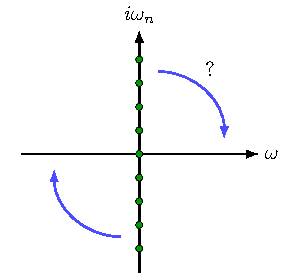
\includegraphics[width=0.3\textwidth]{figs/wick.pdf}} 
	\subfigure[]{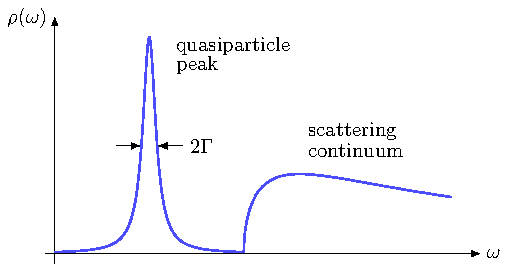
\includegraphics[width=0.55\textwidth]{figs/spectral.pdf}}
	\caption[Analytic continuation and spectral function]{(a) The problem of analytic continuation from discrete imaginary Matsubara frequencies $\omega_n$ to real frequencies $\omega$. (b) Sample spectral function $\rho(\omega,\bm{p}=0)$ featuring a broadened mass peak and a scattering continuum.}
	\label{fig:spectral-properties}
\end{figure}